\chapter{Project Objectives and Specifications}
The project's purpose is to help non-expert users interested in social media analysis to get relevant and reliable information regarding specific concepts. 

\section{Web architecture}
A web architecture is preferable as a modern-day alternative to installable applications. The fast evolution of mobile devices has pushed web developers to segregate User Interfaces from Backend implementations, permitting devices to seamlessly connect to the same under the hood implementation without much development cost and overhead. Communication via REST services is crucial in this concern. Beyond user preference towards such applications, a web architecture presents even more advantages:

\begin{itemize}
\item virtually infinite space extensible with storage backends such as AWS3 or Google Cloud
\item scalability and outsourcing of time-costly services such as getting stream histories
\item database distribution over nodes
\item easily available documentation and integration throughout the development process
\end{itemize} 

Using a web framework eases development even more so and presents security advantages such as stable features, packages and quick patches in the odd case of a security breach. Plugging in services is also considered in the project's context, with handling of specific use cases done in separate managers, loosely coupled with the Model-View-Controller architecture.

\subsection{Data storage}
Since scalability and distribution are a must for a large-scale stream analysis project, data storage should be handled using a method which supports such breakdown while still remaining query-efficient. NoSQL databases are a popular choice for such implementation. The correspondence between the database storage backend and the model part of the application should also be loosely coupled, allowing for the possibility of switching between database backends if the need arises.

Big players in the field of non-relational databases are obvious possible choices: HBase, Cassandra, MongoDB, CouchDB, etc.

\section{ATHENA breakdown}
This thesis is based on the ATHENA original project, which comprises different pipeline steps in acquiring and analysing Twitter feeds:

\begin{itemize}
\item Harvesting: acquisition of collections of related Twitter statuses, by hashtag and dates (start and end).
\item Enhancement: basic analysis of a single harvest with classical unsupervised algorithms
\item Normalisation and Analysis: comparative analysis of harvests
\end{itemize}

\subsection{Twitter as data source}
For the development of this project, I chose to only implement one social media backend as data source. Twitter was the choice, since the character limit they impose is a great asset in regards of data processing: First of all, the classical data analysis pipeline deals with special cases such as documents of different lengths providing unusual skewing to the data set. Another advantage of Twitter is the prevalence of the hashtag model, which has failed to catch on with Facebook to the same degree. This means that statuses basically come out of the box already tagged for content.

Twitter is arguably the second most popular social media platform at the time, gaining on a large number of users even before the mobile device explosion, by integrating with telephone service providers to facilitate posting through SMS. Its 140 character limit makes for a good spin, which has pushed Twitter into a more textual realm than its more successful counterpart, Facebook. The platform is largely popular in the United States and especially in the entertainment domain\footnote{https://en.wikipedia.org/wiki/Twitter}, with the most popular Twitter accounts belonging to celebrities.

It notably also has a history of being the "go to" source for data analysis, after the United States' current president Barrack Obama purportedly used it in his 2008 campaign as one of the principal media outlets, choosing to have a strong Twitter presence, akin to advertisement presence of past candidates.

In short, although this approach is social platform-independent, Twitter was chosen even from the specifications step of this project for a clear start towards the data mining part.

\subsubsection{Fetching data through asynchronous jobs}
Since most social media platforms communicate with external applications via REST APIs with rate limits, the project's structure should include asynchronous modules. In this way, the user will be able to send an API-intensive job for queueing and asynchronous processing, without hindering their overall experience of using the application. This becomes apparent in the Harvesting part.

\subsection{Harvesting}
If we interpret ATHENA as a classical pipeline, then it becomes clear that the Harvesting part is the acquisition part. In order to perform analysis on data, it must first be fetched according to predefined rules and user options. Being time-intensive, these jobs must be designed asynchronously, following a FIFO model.

Figure \ref{fig:harvestpipe1} represents the conceptual model of data acquisition, starting from a collection of grouped documents (in our case they will be collections of statuses with a common hashtag). The Harvest manager handles sending asynchronous jobs via a FIFO queue towards a Consumer-type Harvesting job, represented as black box and further detailed in Figure \ref{fig:harvestpipe}. It is important to note that this pipeline is not in any way adjusted to the domain or the particular API platform; the only constraint we impose is that of periodically checking for compliance to rate limits. Social APIs usually limit requests either by number of requests or requested data size per unit of time. It is therefore a good idea to consider if any limitations alter our pipelines before starting on implementations.

\begin{figure}[ht]
    \centering
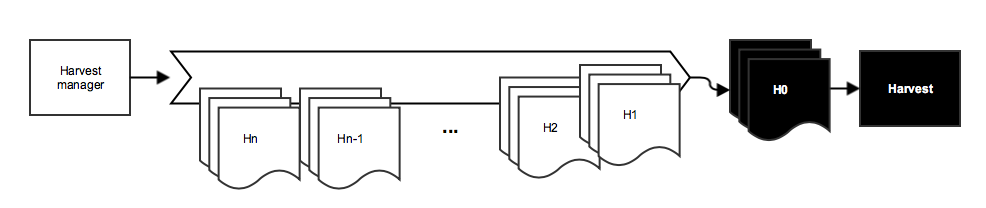
\includegraphics[width=\columnwidth]{img/harvestpipe1.png}
    \caption{Harvesting pipeline}
    \label{fig:harvestpipe1}
\end{figure}

\begin{figure}[ht]
    \centering
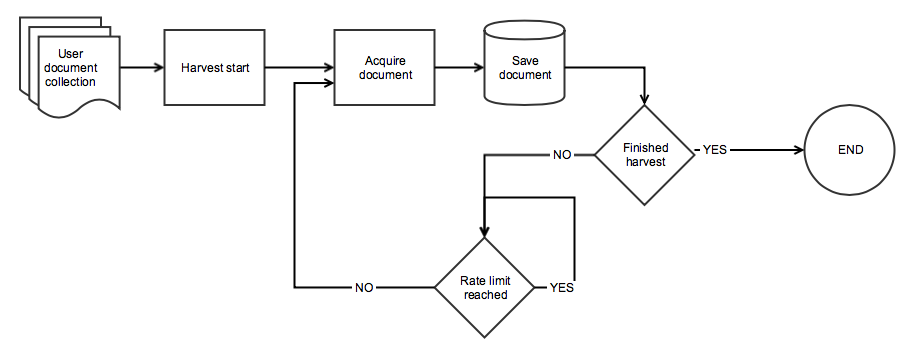
\includegraphics[width=\columnwidth]{img/harvestpipe.png}
    \caption{Harvesting job sub-pipeline}
    \label{fig:harvestpipe}
\end{figure}

\subsection{Enhancement}
As previously stated, it is not of great importance to have the data, but the goal is to obtain meaningful information from it. In this thesis I will refer to "harvests" as per the following definition:

\begin{definition}{}
A Harvest is a collection of documents related by contant, containing a token T and spanning from a start date and to an end date, which have gone through the harvesting pipeline and are stored for further anaylsis.
\end{definition}

After completing the Harvesting pipeline, resulting harvests are processed using various data extraction algorithms and presented to the user in the Enhancement step. These algorithms each have their own sub-pipelines of transformation, which will be detailed in the Analysis step.

\subsubsection{User contribution modeling}
{\color{red} TODO
}

\subsection{Normalisation and analysis}
{\color{red} TODO
}

\section{Non-functional requirements}
I am much concerned with the user's perspective in developing this application. As explained previously, one of the main objectives of this application is undoubtedly to be as simple to use as possible, to benefit non-expert users.

Firstly, I believe that a familiar and streamlined user experience should be implemented. The UI should have componenents found in most web application nowadays, in order to seem aproachable. The customisation options should also be loaded without input from the user, so that things like algorithm choices and parameters should stay hidden. Non-expert users do not know what \emph{Tfidf Vectorizer} or \emph{KMeans clustering} means, all they care about is to have some paplable results to their queries. In short, it is in the benefit of the non-expert users, which I target through this application, to have as little inputs, panels and buttons to figure out.

Besided the look and feel, users will also be interested in having a fast and reliable application. Exceptions and possible bugs should be properly filtered out and time-consuming jobs moved as per Figure \ref{fig:harvestpipe} to asynchronous jobs.